% Created 2024-07-23 Tue 11:42
% Intended LaTeX compiler: pdflatex
\documentclass[10pt]{article}
% =================================BASE====================================%
\usepackage[left=2cm,right=2cm,top=2cm,bottom=2cm]{geometry} % Marges
\usepackage[T1]{fontenc} % Nécessaire avec FrenchBabel
\usepackage[utf8]{inputenc} % Important pour symboles Francophones, é,à,etc
\usepackage{csquotes} % Recommandé par PDFLatex lors de la compilation. 

% Calligraphie
%\usepackage{pxfonts} % Met le texte ET les maths en Palatino + donne accès à des symboles math
\usepackage{palatino} % Cette commande met seulement le texte en police palatino
\usepackage{lmodern} % Pour les maths? Lmodern pour les maths
% Use lmodern for sans-serif
\usepackage{mathrsfs} % Permet la command \mathscr (Lettres attachées genre) \mathscr(B)

% Bibliographie
%\usepackage[backend=bibtex,style=phys,sorting=ynt]{biblatex}
\usepackage[backend=biber,sorting=ynt,style=authoryear]{biblatex} % N'est pas utilisé par le compilateur org-mode, mais NÉCESSAIRE. Voir le fichier init.el pour changer le style. 
\addbibresource{/home/charlesedouard/Desktop/Travail/Documentation/2023/master-bibliography.bib}


\usepackage{amsmath, amssymb, amsthm} % Symb. math. (Mathmode+Textmode) + Beaux théorèmes.
\usepackage{mathtools,cancel,xfrac} % Utilisation de boîtes \boxed{} + \cancelto{}{}, xfrac
\usepackage{graphicx, wrapfig} % Géstion des figures.
\usepackage{hyperref} % Permettre l'utilisation d'hyperliens.
\usepackage{color} % Permettre l'utilisation des couleurs.
\usepackage{colortbl} % Color tables
\usepackage[dvipsnames]{xcolor} % Couleurs avancées.

% Physique
\usepackage{physics} % Meilleur package pour physicien. 

% Style
\usepackage{lipsum} % For fun
\usepackage{tikz} % Realisation de figures TIKZ.
\usetikzlibrary{arrows.meta,bending} % Arrow heads 
\usepackage{empheq} % Boite autour de MULTIPLE équations
\usepackage{bbding}

% Français
\usepackage[french]{babel} % Environnements en Français.

\usepackage{titling} % Donne accès à \theauthor, \thetitle, \thedate

% ==============================BASE-(END)=================================%





% ================================SETTINGS=================================%
% Pas d'indentation en début de paragraphe :
\setlength\parindent{0pt}
\setlength{\parskip}{0.15cm}

% Tableaux/tabular
% Espace vertical dans les tabular/tableaux
\renewcommand{\arraystretch}{1.2}
% Couleur des tableaux/tabular
% \rowcolors{3}{violet!5}{}

% Couleurs de hyperliens :
\definecolor{mypink}{RGB}{147, 0, 255}
\hypersetup{colorlinks, 
             filecolor=mypink,
             urlcolor=Violet, 
             citecolor=mypink, 
             linkcolor=mypink, 
             anchorcolor=mypink}


% Numéros d'équations suivent les sections :
\numberwithin{equation}{section} 

% Les « captions » sont en italique et largeur limitée
\usepackage[textfont = it]{caption} 
\captionsetup[wrapfigure]{margin=0.5cm}

% Retirer l'écriture en gras dans la table des matières
\usepackage{tocloft}
\renewcommand{\cftsecfont}{\normalfont}
\renewcommand{\cftsecpagefont}{\normalfont}

% Change bullet style
\usepackage{pifont}
\usepackage{enumitem}
%\setlist[itemize,1]{label=\ding{224}}
\setlist[itemize,1]{label=\ding{239}}
\renewcommand{\boxtimes}{\blacksquare}
% ================================SETTINGS=================================%



% ==============================NEWCOMMANDS================================%
% CQFD symbol
\renewcommand{\qedsymbol}{$\hfill\blacksquare$}

% Vecteurs de base :
\newcommand{\nvf}{\vb{\hat{n}}}
\newcommand{\evf}{\vb{\hat{e}}}
\newcommand{\ivf}{\vb{\hat{i}}}
\newcommand{\jvf}{\vb{\hat{j}}}
\newcommand{\kvf}{\vb{\hat{k}}}
\newcommand{\uu}{\vb{u}}
\newcommand{\vv}{\vb{v}}
\newcommand{\ust}{\vb{u}_{\ast}}

% Physics empty spaces 
\newcommand{\short}{\vphantom{pA}}
\newcommand{\tall}{\vphantom{pA^{x^x}_p}}
\newcommand{\grande}{\vphantom{\frac{1}{xx}}}
\newcommand{\venti}{\vphantom{\sum_x^x}}
\newcommand{\pt}{\hspace{1pt}} % One horizontal pt space

% Moyenne numérique entre deux points de grilles. 
\newcommand{\xmean}[1]{\overline{#1}^x}
\newcommand{\ymean}[1]{\overline{#1}^y}
\newcommand{\zmean}[1]{\overline{#1}^z}
\newcommand{\xymean}[1]{\overline{#1}^{xy}}

% Tilde over psi
\newcommand{\tpsi}{\tilde{\psi}}
\newcommand{\tphi}{\tilde{\phi}}

% Nota Bene env : (\ding{89})
%\newcommand{\nb}{$\boxed{\text{\footnotesize\EightStarConvex}\pt \mathfrak{N. B.}}$\hspace{4pt}}
\newcommand{\nb}{\underline{{\footnotesize\EightStarConvex}\pt $\mathfrak{N.B.}$\vphantom{p}}\hspace{3pt}}

\newcommand{\exemple}{
\parbox[center]{2.2cm}{\begin{tcolorbox}[sharp corners, rounded corners=northeast, rounded corners=southeast,
colback=Violet!5, colframe=black,
size=small, width=2cm, left=-0.25pt, bottom=-0.5pt,
arc is angular, arc=2.5mm, boxrule=0.35pt, leftrule=4pt, %bottomrule=1pt,
after={\enskip}] Exemple \end{tcolorbox}}}

\newcommand{\cqfd}{\hfill$\blacktriangleleft$}

% Define the nota bene environment
\usepackage{tcolorbox}
\newtcolorbox{notabene}{
     colback=blue!5,
     colframe=black,
     boxrule=0.5pt,
     arc=2pt,
     left=5pt,
     right=5pt,
     top=5pt,
     bottom=5pt,
}


\newcommand{\cmark}{\ding{52}}
\newcommand{\xmark}{\ding{55}}
% ==============================NEWCOMMANDS================================%



% ==============================PAGE-TITRE=================================%
% Titlepage 
\newcommand{\mytitlepage}{
\begin{titlepage}
\begin{center}
{\Huge \thesubtitle \par}
\vspace{2cm}
{\Huge \MakeUppercase{\thetitle} \par}
\vspace{2cm}
RÉALISÉ DANS LE CADRE\\ D'UN PROJET POUR \par
\vspace{2cm}
{\Huge ISMER--UQAR \par}
\vspace{2cm}
{\thedate}
\end{center}
\vfill
Rédaction \\
{\theauthor}\\
\url{charles-edouard.lizotte@uqar.ca}\\
ISMER-UQAR\\
Police d'écriture : \textbf{CMU Serif Roman}
\end{titlepage}
}
% ==============================PAGE-TITRE=================================%



% =================================ENTÊTE==================================%
\usepackage{fancyhdr}
\pagestyle{fancy}
\setlength{\headheight}{13pt}
\renewcommand{\headrulewidth}{0.025pt} % Ligne horizontale en haut

\fancyhead[R]{\textit{\thetitle}}
\fancyhead[L]{\ \thepage}
\fancyfoot[R]{\textit{\theauthor}}
\fancyfoot[L]{}
\fancyfoot[C]{} 
% =================================ENTÊTE==================================%
\author{Charles-Édouard Lizotte}
\date{21/04/2023}
\title{Carnet de bord, Université McGill}
\newcommand{\thesubtitle}{Contrat Été 2023}
\hypersetup{
 pdfauthor={Charles-Édouard Lizotte},
 pdftitle={Carnet de bord, Université McGill},
 pdfkeywords={},
 pdfsubject={},
 pdfcreator={Emacs 27.1 (Org mode 9.6.7)}, 
 pdflang={French}}
\begin{document}

\mytitlepage
\tableofcontents\newpage


\section{MUDPACK}
\label{sec:org5c7b6dc}
\subsection{Mise en contexte}
\label{sec:org46cf6ab}


\begin{wrapfigure}[17]{r}{0.41\textwidth} \vspace{-\baselineskip}
\centering
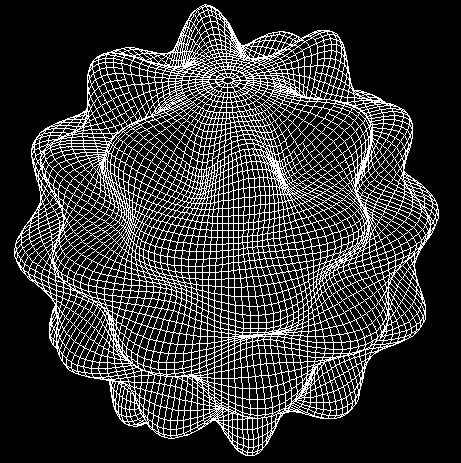
\includegraphics[width=0.38\textwidth]{figures/logos/SPHERE.png}
\caption{\label{fig:org17336ba}Logo MUDPACK}
\end{wrapfigure}

\textbf{N.B.} Nous sommes jeudi le 13 avril et je commence enfin à \emph{jouer} avec la suite MUDPACK   \autocite{adams1989mudpack}.
Malheureusement, je n'ai pas pu débuter cette tâche pour l'instant.
Jusqu'à maintenant, les problèmes de modes barotropes et baroclines ont été plus graves que je croyais, mais tout semble enfin fonctionner.
Les valeurs propres calculées analytiquement sont semblables à celles calculées numériquement. \bigskip

MUDPACK \autocite{adams1989mudpack} est une suite FORTRAN en développement depuis les années 70.
Son usage principal est de résoudre des équations différentielles partielles elliptiques, comme dans le cas qui nous intéresse.
Elle fait partie des \href{https://arc.ucar.edu/knowledge\_base/71991310}{NCAR Classic Libraries for Geophysics} et sont encore régulièrement utilisées par la communauté géophysique.
L'accronyme NCAR fait référence à \emph{National Center For Atmospheric Research}, on doute donc que la communauté géophysique tient les suite FORTRAN à bout de bras.\bigskip

Toutes ces suites FORTRAN sont disponibles sur le \href{https://github.com/NCAR/NCAR-Classic-Libraries-for-Geophysics}{GitHub de NCAR} et on remarque qu'en date de la l'écriture de ce carnet, ces sous-routines ont été mises à jour il y a moins de deux ans.
Je trouve ça exceptionnel pour un langage de programmation que beaucoup de gens trouvent « vieux jeux » et même désuet.
Bref, contre toutes attentes, les « excursions » numériques de David et Louis-Philippe commencent à me plaire.

\subsection{Téléchargement de la suite MUDPACK}
\label{sec:org96610f2}
Avant de débuter, on se doute qu'il faut -- au même titre que la suite LAPACK -- installer le module Fortran et lui assigner un \emph{PATH}, car il n'est probablement pas déjà installé sur les versions usuelles de Ubuntu.
À première vue, la suite MUDPACK est introuvable sur la toile et il existe très peu de documentation, mis à part quelques pages GitHub personnelles.
Comme pour l'installation de LAPACK, je me demandais s'il y avait un moyen d'installer une archive avec une commande Debian du type
\begin{verbatim}
  >>> sudo apt-get install libmudpack etc etc
\end{verbatim}
Pourtant, non : Il n'existe tout simplement pas d'archive MUDPACK pour langage FORTRAN disponible sur les répertoires en ligne de l'installateur Aptitude.
Devant ce problème, j'ai demandé l'aide de notre nouvel ami : ChatGPT,  pour me trouver un moyen de l'installer.
D'abord, ChatGPT a trouvé quelques versions du module mais ces dernières étaient purement obsolètes, dont celle d'un de ses développeurs vedette, \href{https://netlib.org/utk/people/JackDongarra/}{Jack Dongarra}.
Un personnage fort intéressant d'ailleurs qui mériterait sa propre section.
Comme le fichier \emph{tar} sur lequel ChatGPT pointait était désuet, je lui ai surtout demandé de m'orienter sur le chemin à prendre pour télécharger ce genre de librairie FORTRAN.
Je ne suis pas très accoutumé à télécharger et à travailler avec des fichiers \emph{tar}, mais les étapes étaient simple à suivre.\newline

Je suis donc revenu à l'archive GitHub précédente (celle de NCAR) qui contenait une \href{https://github.com/NCAR/NCAR-Classic-Libraries-for-Geophysics}{version à jour}  de tous les librairies d'algèbre linéaire, dont \href{https://github.com/NCAR/NCAR-Classic-Libraries-for-Geophysics/tree/main/MudPack}{MUDPACK}.
Une fois sur place, il est très simple de télécharger le fichier \emph{tar} dans nos \emph{Documents} à l'aide de la commande \emph{wget}, soit
\begin{verbatim}
  >>> cd ~\Documents
  >>> wget https://github.com/NCAR/NCAR-Classic-Libraries-for-Geophysics/blob/main/MudPack/mudpack
  5.0.1.tar.gz?raw=true -O mudpack5.0.1.tar.gz
\end{verbatim}
où le lien est celui obtenu en cliquant « \textbf{View Raw} » sur le fichier dans l'archive GitHub.
Une fois téléchargé, on peut ouvrir le \emph{tar} à l'aide des commandes
\begin{verbatim}
  >>> gunzip mudpack5.0.1.tar.gz
  >>> tar xvf mudpack5.0.1.tar
  >>> cd mudpack5.0.1
\end{verbatim}
comme il est conseillé de faire dans le README en ligne.

\subsection{Installation et compilation de la suite MUDPACK}
\label{sec:orgf936c36}
Il sera nécessaire de constuire et compiler la suite à l'aide d'un \emph{Makefile}.
Nous allons donc modifer le fichier \emph{bash} \emph{make.inc} qui construira un \emph{Makefile} à l'aide des bons compilateurs.
\begin{enumerate}
\item En premier lieu, on remplace \emph{-fmod=} par \emph{-J} partout. La commande \emph{fmod} est désuette avec tous les compilateurs modernes, c'est une commande qui dit dans quel dossier mettre le modules issus de la compilation.
\item Deuxièmement, on remplace toutes les mentions  à « pgf90 » et « g95 » par « gfortran », tout simplement parce que c'est notre compilateur.
\end{enumerate}

Au final, le fichier devrait avoir une section principale qui ressemble à

\begin{verbatim}
ifeq ($(UNAMES),Linux)

  PGI := $(shell gfortran 2>&1)

  ifeq ($(PGI),gfortran-Warning-No files to process)

    F90 := gfortran -module ../lib -I../lib
    CPP := gfortran -E

  else

    F90 := gfortran -DG95 -g -J../lib -I../lib 
    CPP := gfortran -E -DG95

  endif

  MAKE := gmake
  AR := /usr/bin/ar

endif
\end{verbatim}

Bon! C'est enfin le temps de compiler! Dans le dossier principal, on exécute la commande \emph{gmake},
\begin{verbatim}
  >>> gmake
\end{verbatim}
Cette action devrait exécuter plusieurs centaines de lignes dans l'invite de commande, mais n'ayons pas peur.
L'important à retenir : un nouveau fichier, soit une \href{https://docs.oracle.com/cd/E19957-01/805-4940/6j4m1u7ov/index.html}{librairie statique}, devrait avoir été crée dans le dossier \emph{lib} : \emph{libmudpack.a}.
Ce fichier est une archive, on peut donc s'en servir et le lier à notre code.
De manière générale, les librairies se retrouvent dans le répertoire des librairies, soit le même que LAPACK.
C'est donc à cet endroit que nous allons créer un répertoire pour la librairie MUDPACK,
\begin{verbatim}
  >>> cd /usr/lib/x86_64-linux-gnu/
  >>> sudo mkdir mudpack
  >>> cd mudpack
\end{verbatim}
On copie la librairie \emph{libmudpack.a} juste ici :
\begin{verbatim}
  >>> sudo cp ~/Documents/mudpack5.0.1/lib/libmudpack.a .
\end{verbatim}

Notre librairie maintenant installée, il faut lier notre compilateur à cette nouvelle librairie.
Dans notre exécutable \emph{bash}, on devrait avoir quelque chose qui ressemble à
\begin{verbatim}
  #!/bin/bash
  mudpack_path=/usr/lib/x86_64-linux-gnu/mudpack
  lapack_path=/usr/lib/x86_64-linux-gnu/lapack
  gfortran -o poisson-exec mudpack-test.f90 -L$mudpack_path -lmudpack
\end{verbatim}
S'il n'y pas pas d'erreur lors de la compilation du code, il est possible de vérifier si la librairie a bien été liée à l'aide de la commande \emph{ldd} sur notre exécutable.
Cette commande nous fait essentiellement mention de toutes les librairies utilisées par l'exécutable.
\begin{verbatim}
  >>> ldd poisson-exec
  linux-vdso.so.1 (0x00007ffd39130000)
  libgfortran.so.5 => /lib/x86_64-linux-gnu/libgfortran.so.5 (0x00007fa3edddb000)
  libm.so.6 => /lib/x86_64-linux-gnu/libm.so.6 (0x00007fa3edcf4000)
  libc.so.6 => /lib/x86_64-linux-gnu/libc.so.6 (0x00007fa3edacc000)
  libquadmath.so.0 => /lib/x86_64-linux-gnu/libquadmath.so.0 (0x00007fa3eda84000)
  libgcc_s.so.1 => /lib/x86_64-linux-gnu/libgcc_s.so.1 (0x00007fa3eda64000)
  /lib64/ld-linux-x86-64.so.2 (0x00007fa3ee0fc000)
\end{verbatim}

\section{Conditions frontières et schéma numérique}
\label{sec:org56fffa7}
\subsection{Mise en contexte}
\label{sec:org26855ac}
\begin{wrapfigure}[20]{r}{0.45\textwidth}
\vspace{-\baselineskip}
\centering
\begin{tikzpicture}[scale=2.7]
% Grille : 
\draw[step=1.0,black,dotted] (1.,1.) grid (3.25,3.25);
% Flèches en v : 
\foreach \x in {1,2}
\foreach \y in {1,2,3}
{
    \draw [-{latex},red]
              (\x + 0.5, \y - 0.1 ) --
              (\x + 0.5, \y + 0.1);
    \draw [] (\x + 0.5, \y + 0.0) node [red,right] {$v\pt [\x,\y]$};
}
% Flèches en u :
\foreach \x in {1,2,3}
\foreach \y in {1,2}
{
    \draw [-{latex},blue](\x - 0.1 , \y + 0.5 ) --
              node [below,blue] {$u\pt[\x,\y]$}
              (\x + 0.1, \y + 0.5);
}
% Points aux coins :
\foreach \x in {1,2,3}
\foreach \y in {1,2,3}
{
\fill [black] (\x, \y) circle (0.5pt);
}
% Milieux :
\foreach \x in {1,2}
\foreach \y in {1,2}
{\draw (\x+0.5,\y+0.5) node [] {$\qty[\pt\x,\y\pt]$} ;}
% Flèches
\node [] at (1.5,0.75) (dx1) {$\Delta x$};
\draw [-{latex}|] (dx1) -- (1,0.75);
\draw [-{latex}|] (dx1) -- (2,0.75);
\node [] at (0.70,1.5) (dy1) {$\Delta y$};
\draw [-{latex}|] (dy1) -- (0.70,1);
\draw [-{latex}|] (dy1) -- (0.70,2);
\end{tikzpicture}
\caption{\label{orgdb17e08}Représentation de la grille numérique utilisée pour le modèle en eau peu profonde (type \href{https://en.wikipedia.org/wiki/Arakawa\_grids}{Arakawa-C} )}
\end{wrapfigure}

Pour débuter, nous voulons rajouter des murs aux frontières de notre expérience numérique.
Par contre, ceci nous empêche d'emprunter le solveur elliptique précédemment utilisé dans le modèle à deux couches.
Ce dernier fonctionnait avec des transformées de Fourrier, il aurait donc fallu créer des réflexions en x et y pour rendre les frontières continues sur un plus grand domaine.
Et les réflexions auraient été inverses dans certains cas.
Par exemple, la réflexion en \(x\) du courant en \(v\) aurait été une réflexion négative, tandis que la réflexion en \(x\) du courant en \(u\) aurait été une réflexion positive pour s'assurer de la continuité dans les 4 quadrants.
De plus, on aurait surement souffert du phénomène de Gibbs aux discontinuités.
C'est pourquoi nous avons oublié cette idée.\bigskip

Comme mentionné précédemment, nous utiliserons le solveur elliptique de la suite MUDPACK \autocite{adams1989mudpack}.
Ce solveur utilise plutôt des fonctions de Green ou une technique de relaxation pour résoudre les équations différentielles partielles du second ordre.
Par contre, il faudra ajuster les conditions limites de sorte à ce que le courant, sa dérivée première et sa dérivée seconde soient définit aux frontières.\bigskip

\textbf{N.B.} Mentionnons que le nombre de conditions frontières nécessaires augmente directement avec l'ordre de l'équation différentielle que nous tentons de résoudre.

\subsection{Conditions frontière sur les courants (No normal flow)}
\label{sec:org4fa8708}
Pour les courants qui traversent les murs, on applique la condition \emph{no normal flow}.
La condition \emph{no normal flow} est une condition de type Dirichlet qui est caractérisée par un courant normal nul aux frontières, bref comme si le fluide \emph{adhérait} aux murs.
C'est donc une condition d'imperméabilité.
Mathématiquement, la condition se traduit par
\begin{equation}
\uu \cdot \nvf =0,
\end{equation}
où \(\nvf\) est le vecteur normal à la frontière.
Numériquement, on peut énoncer que sur une grille cartésienne la condition \emph{no normal flow} symbolise
\begin{subequations}
\begin{align}
  &&(\text{Frontières verticales}) && u\pt[1\pt,:] = 0 && \text{et} && u\pt[:\pt,nx] = 0,&& \\
  &&(\text{Frontières horizontales}) && v\pt[:\pt,1] = 0 && \text{et} && v\pt[:\pt,ny] = 0,&&  
\end{align}
\end{subequations}

\textbf{N.B.} Si nous utilisons des points fantômes, alors on peut étendre les extrémités des frontières et affirmer que ces derniers sont reliés par les relations
\begin{subequations}
\begin{align}
(\text{Courant }u) &&  u\pt[\pt:\pt,0] = u\pt[\pt:\pt,1] && \text{et} && u\pt[\pt:\pt,ny+1] &= u\pt[\pt:\pt,ny],&&\\
(\text{Courant }v) &&  v\pt[0,\pt:\pt] = v\pt[1,\pt:\pt] && \text{et} && v\pt[nx+1,\pt:\pt] &= v\pt[nx,\pt:\pt].&&
\end{align}
\end{subequations}

\subsection{Conditions frontières sur la dérivée première (Free slip condition)}
\label{sec:org9362732}
Avant tout, mentionnons qu'on fait régulièreement référence à un concept appelé la \emph{no slip condition}.
Cette condition se caractérise par l'absence de courant tangeant au mur.
Comme le courant normal aux frontières est généralement nul dans les cas à l'étude (\emph{no normal flow}), la \emph{no slip condition} réfère généralement au fait qu'aucun fluide ne bouge au mur.\bigskip

Par contre, on s'intéresse aujourd'hui à la \emph{free slip condition}.
La \emph{free slip condition} tient à l'hypothèse que la couche limite est si petite qu'on peut essentiellement l'ignorer, ce qui est souvent le cas pour l'étude des fluides à grande échelle.
Concrétement, il n'y a \href{https://physics.stackexchange.com/questions/383096/understanding-free-slip-boundary-condition\#:\~:text=On\%20the\%20other\%20hand\%2C\%20the,the\%20tangential\%20component\%20is\%20unrestricted.}{pas de contrainte de cisaillement au mur}, de sorte que
\begin{align}
\label{eq:org39d524e}
&&\eval{\qty(\boldsymbol{\tau}_x = \mu \pdv{u}{y})\pt }_{\pt\{xi,xf\}} = 0\pt, && \text{et} &&
  \eval{\qty(\boldsymbol{\tau}_x = \mu \pdv{u}{y})\pt }_{\pt\{yi,yf\}} = 0\pt. &&
\end{align}
où \(\mu\) est la viscosité \autocite{tan2018applying}.
Ainsi, l'expression \ref{eq:org39d524e} force la condition frontière sur la dérivée première à satisfaire 
\begin{equation}
\boxed{\hspace{0.7cm}\eval{\pdv{v}{x}\pt }_{\pt\{xa,xf\}} = 0\pt\ \forall\ y,\hspace{1.3cm} \text{et} \hspace{1.3cm} \eval{\pdv{u}{y}\pt }_{\pt \{yi,yf\}} = 0\pt\ \forall\ x.\hspace{0.7cm}\bigno}
\end{equation}


\subsection{Calcul de la dérivée seconde en présence de murs}
\label{sec:org797a919}
Pour calculer la dérivée seconde, on a besoin de trois points, de sorte que la courbure de notre champ est donnée par
\begin{equation}
\pdv[2]{u}{x} [i,:\pt] = \frac{u\pt[i-1,:\pt] + u\pt[i+1,:\pt] -2u\pt[i,:\pt]}{\Delta x^2}.
\end{equation}
Et dans notre schéma numérique, la seconde dérivée se positionne au même point que la quantité choisie, le courant en \(u\) dans notre cas.\bigskip

Par contre, aux frontières, une partie de cette information est cachée derrière le mur.
Il faut donc trouver un moyen détourné d'obtenir la dérivée seconde.
David a proposé une méthode assez intéressante impliquant les série de Taylor.
On peut réaliser deux séries autour des points aux frontières normales.
Par exemple, on peut prendre \(u\pt[1,:]\) et étendre notre série autour de \(u\pt[2,:]\) et \(u\pt[3,:]\) pour obtenir
\begin{subequations}
\begin{align}
&u[2,:] = u[1,:] + (\Delta x)\ u'[1,:] + (\Delta x)\frac{u''[1,:]}{2} + \order{3},\\
&u[3,:] = u[1,:] + (2\Delta x)u'[1,:] + (2\Delta x)^2\frac{u''[1,:]}{2} + \order{3}.
\end{align}
\end{subequations}
Maintenant, on soustrait les deux équations de sorte à éliminer \(u[1,:]\) et retrouver la dérivée suivante, soit
\begin{equation}
\underbrace{u[3,:] - u[2,:]}_{u'[2,\pt:\pt]} = \Delta x\ u'[1,:] +  \frac{3\Delta x^2}{2} u''[1,:]
\end{equation}
et on aboutit à l'expression
\begin{equation}
\boxed{\hspace{0.3cm}
u''[1,:] = \frac{2}{3\Delta x} \big(\vphantom{()}\pt u'[2,:] - u'[1,:]\pt \big).
\hspace{0.3cm}}
\end{equation}
Le même principe est applicable à chaque frontière et dans chaque direction.\newpage

\subsection{Étude des conditions frontières et lien avec MUDPACK}
\label{sec:orgeee1ce5}
\begin{wrapfigure}[14]{r}{0.5\textwidth}
\centering
\begin{tikzpicture}[scale=0.8]
   % Lignes
   \filldraw[black!3] plot[smooth, tension=0.7] coordinates {(-3.,0.5) (-2,3) (1.5,3) (4,3.5) (5,2.5) (5.3,-1) (0,-0.5) (-2.6,-2) (-3.,0.5)};
   \draw[blue,thick]  plot[smooth, tension=0.7] coordinates {(-3.,0.5) (-2,3) (1.5,3) (4,3.5) (5,2.5)};
   \draw[red,thick]  plot[smooth, tension=.7] coordinates { (5,2.5) (5.3,-1) (0,-0.5) (-2.6,-2) (-3.,0.5)};
   % Points
   \filldraw[black] (5,2.5) circle (2pt);
   \filldraw[black] (-3.,0.5) circle (2pt);
   % Noms des courbes
   \draw [red]  (-2.3,-1) node {\large$C_1$};
   \draw [blue] (3.8,2.8) node {\large$C_2$};
   \draw [black!70] (1.6,1.2) node {\Large$\Omega(C)$};
   % Conditions frontières
   \draw (0.6,-1.2) node {\large$\phi|_{C_1} = \phi_0$};
   \draw (-1.1,2.1) node {\large $\eval{\pdv{\phi}{n}}_{C_2}\hspace{-0.3cm}= f$};
\end{tikzpicture}
\caption{\label{org33e6c77}Condition frontière mixte autour d'une région \(\Omega\) borné par la courbe \(C = C_1\cup C_2\).}
\end{wrapfigure}

Pour chaque frontière, il est possible d'appliquer une condition différente sur la fonction \(\phi\).
L'usager a pour sa part trois choix : 
\begin{itemize}
\item Le domaine est périodiques sur la frontière (\emph{iparm(2) = 0});
\item La fonction à déterminer (\(\phi\)) est définit aux frontières (Dirichlet) (\emph{iparm(2) = 1});
\item On spécifie la valeur de la dérivée normale à la frontière (Neumann) et/ou on définit des conditions frontières mixtes (\emph{iparm(2) = 2}).\bigskip
\end{itemize}

Dans le cas à l'étude, une condition frontière de type Neumann est préférable.
Il est possible de définir des conditions frontières mixtes (Neumann et Dirichlet), mais ce ne sera pas nécessaire pour notre grille.\bigskip

Prenons en exemple la frontière ouest.
Toujours selon la documentation de MUDPACK, les conditions frontière mixtes ont la forme,
\begin{equation}
\pdv*{\phi}{x} + \alpha(y)*\phi(xa,y) = f(y) \hspace{0.5cm} \forall \hspace{0.3cm} y\ \in \ \qty[y_i\pt,y_f], 
\end{equation}
où \(\phi(x,y)\) est la solution à déterminer.
Les fonctions \(\alpha(y)\) et \(f(y)\) restent donc à déterminer pour notre problème aux conditions frontières.\bigskip

On sait que l'évolution du fluide est décrit par le système d'équations
\begin{subequations}
\begin{align}
u\pt (\pt t+1)  = u(t) + \Delta t \pt G_x\pt(x,y,t) + \pdv*{\phi}{x}, \label{eq:evolution}\\
v\pt (\pt t+1)  = v(t) + \Delta t \pt G_y\pt(x,y,t) + \pdv*{\phi}{y},
\end{align}
\end{subequations}
où les termes \(G_{x,y}\) sont des termes valisent qui englobent tout le côté droit de nos équations du mouvement dans chaque direction (Coriolis, advection horizontale, gradient de la fonction de Bernouilli, etc).\bigskip

Au mur ouest, on impose la condition d'imperméabilité (\emph{no normal flow}) sur l'équation \ref{eq:evolution} de sorte que \(u(x_0,y,t) = 0\) et
\begin{equation}
\eval{\pdv{\phi}{x}}_{x_0} = -\Delta t \pt G_x\pt(x_0,y,t),
\hspace{0.5cm}\Longrightarrow\hspace{0.5cm}
\boxed{\hspace{0.2cm}f(y) = -\Delta t \pt G_x\pt(x,y,t) \hspace{0.35cm}\&\hspace{0.35cm} \alpha(y) = 0 \hspace{0.2cm}}
\end{equation}

Un lecteur avisé serait tenté de vérifier si \(G_x = 0\) pour se simplifier la vie.
Vérifions l'état des fonctions \(G_{x,y}\) à la frontière ouest,
\begin{equation}
G_x(x_0,y) = \underbrace{\cancelto{0}{u\cdot\qty(\pdv{u}{x})} + \cancelto{0}{v\cdot\qty(\pdv{u}{y})}}_\text{Advection}
\underbrace{\ +\ f v \ \bigno}_\text{Coriolis}
\underbrace{\ +\ \frac{\tau_x}{\rho_o}\ \bigno}_\text{Vent}
\underbrace{\ +\ D_x. \bigno}_\text{Dissip.}
\end{equation}
On peut aisément retirer les termes d'avection, étant donné que \({u(x_0,y)=\pdv*{u}{y}|_{x_0} = 0\ \forall\ y}\).
Malheureusement, les termes \({G_{x,y} \neq 0}\).
Par contre, on note qu'il y aura l'établissement d'un équilibre entre les termes sources et le gradient de pression \(\gradient{\phi}\).

\printbibliography
\end{document}